\documentclass[sigconf,table,10pt]{acmart}

\usepackage{algpseudocode}
\usepackage{algorithm}
\usepackage{algorithmicx}
\usepackage{verbatim}
\usepackage{mathtools}
\usepackage{multirow}
\usepackage{subcaption}
\usepackage{colortbl}
\usepackage{balance}
\usepackage{extarrows}

\usepackage{tikz}
\usetikzlibrary{automata,positioning}

\definecolor{lightgray}{gray}{0.9}


%\def\BibTeX{{\rm B\kern-.05em{\sc i\kern-.025em b}\kern-.08em
%	T\kern-.1667em\lower.7ex\hbox{E}\kern-.125emX}}

\usepackage{booktabs} % For formal tables


\newlength\Origarrayrulewidth

% horizontal rule equivalent to \cline but with 2pt width
\newcommand{\Cline}[1]{%
	\noalign{\global\setlength\Origarrayrulewidth{\arrayrulewidth}}%
	\noalign{\global\setlength\arrayrulewidth{3pt}}\cline{#1}%
	\noalign{\global\setlength\arrayrulewidth{\Origarrayrulewidth}}%
}

% draw a vertical rule of width 2pt on both sides of a cell
\newcommand\Thickvrule[1]{%
	\multicolumn{1}{!{\vrule width 2pt}c!{\vrule width 2pt}}{#1}%
}

% draw a vertical rule of width 2pt on the left side of a cell
\newcommand\Thickvrulel[1]{%
	\multicolumn{1}{!{\vrule width 2pt}c}{#1}%
}

% draw a vertical rule of width 2pt on the right side of a cell
\newcommand\Thickvruler[1]{%
	\multicolumn{1}{c!{\vrule width 2pt}}{#1}%
}

%%
%% \BibTeX command to typeset BibTeX logo in the docs
\AtBeginDocument{%
	\providecommand\BibTeX{{%
			\normalfont B\kern-0.5em{\scshape i\kern-0.25em b}\kern-0.8em\TeX}}}

%% Rights management information.  This information is sent to you
%% when you complete the rights form.  These commands have SAMPLE
%% values in them; it is your responsibility as an author to replace
%% the commands and values with those provided to you when you
%% complete the rights form.

\copyrightyear{2021}
\acmYear{2021}
\setcopyright{acmcopyright}\acmConference[GRADES-NDA'21]{Joint Workshop on Graph Data Management Experiences \& Systems (GRADES) and Network Data Analytics (NDA)}{June 20, 2021}{Xi'an, Shaanxi, China}
\acmBooktitle{Joint Workshop on Graph Data Management Experiences \& Systems (GRADES) and Network Data Analytics (NDA), June 20, 2021, Xi'an, Shaanxi, China}
\acmPrice{15.00}
\acmDOI{}
\acmISBN{}


%%
%% Submission ID.
%% Use this when submitting an article to a sponsored event. You'll
%% receive a unique submission ID from the organizers
%% of the event, and this ID should be used as the parameter to this command.
%%\acmSubmissionID{123-A56-BU3}

%%
%% The majority of ACM publications use numbered citations and
%% references.  The command \citestyle{authoryear} switches to the
%% "author year" style.
%%
%% If you are preparing content for an event
%% sponsored by ACM SIGGRAPH, you must use the "author year" style of
%% citations and references.
%% Uncommenting
%% the next command will enable that style.
%%\citestyle{acmauthoryear}

\newtheorem{mytheorem}{Theorem}
\newtheorem{myproposition}{Proposition}

\newcommand{\ltz}{$< 1$}

\algtext*{EndWhile}% Remove "end while" text
\algtext*{EndIf}% Remove "end if" text
\algtext*{EndFor}% Remove "end for" text
\algtext*{EndFunction}% Remove "end function" text

%%
%% end of the preamble, start of the body of the document source.
\begin{document}
	\fancyhead{}
	
	%%
	%% The "title" command has an optional parameter,
	%% allowing the author to define a "short title" to be used in page headers.
	\title[]{Context-Free Path Querying with All-Path Semantics by Matrix Multiplication}
	
	%%
	%% The "author" command and its associated commands are used to define
	%% the authors and their affiliations.
	%% Of note is the shared affiliation of the first two authors, and the
	%% "authornote" and "authornotemark" commands
	%% used to denote shared contribution to the research.
	
	
	\author{Rustam Azimov}
	\email{rustam.azimov19021995@gmail.com}
	\affiliation{
		\institution{Saint Petersburg State University}
		\streetaddress{7/9 Universitetskaya nab.}
		\city{St. Petersburg}
		\country{Russia}
		\postcode{199034}
	}
	\affiliation{
		\institution{JetBrains Research}
		\streetaddress{Primorskiy prospekt 68-70, Building 1}
		\city{St. Petersburg}
		\country{Russia}
		\postcode{199034}
	}

\author{Ilya Epelbaum}
\email{iliyepelbaun@gmail.com}
%\authornote{}
\affiliation{
	\institution{Saint Petersburg State University}
	\streetaddress{7/9 Universitetskaya nab.}
	\city{St. Petersburg}
	\country{Russia}
	\postcode{199034}
}
\affiliation{
	\institution{JetBrains Research}
	\streetaddress{Primorskiy prospekt 68-70, Building 1}
	\city{St. Petersburg}
	\country{Russia}
	\postcode{199034}
}
	
	
	\author{Semyon Grigorev}
	\email{s.v.grigoriev@spbu.ru}
	\email{semyon.grigorev@jetbrains.com}
	\orcid{0000-0002-7966-0698}
	\affiliation{
		\institution{Saint Petersburg State University}
		\streetaddress{7/9 Universitetskaya nab.}
		\city{St. Petersburg}
		\country{Russia}
		\postcode{199034}
	}
	\affiliation{
		\institution{JetBrains Research}
		\streetaddress{Primorskiy prospekt 68-70, Building 1}
		\city{St. Petersburg}
		\country{Russia}
		\postcode{199034}
	}
	
	%%
	%% By default, the full list of authors will be used in the page
	%% headers. Often, this list is too long, and will overlap
	%% other information printed in the page headers. This command allows
	%% the author to define a more concise list
	%% of authors' names for this purpose.
	\renewcommand{\shortauthors}{Terekhov, Khoroshev, Azimov, Grigorev}
	
	%
	% The abstract is a short summary of the work to be presented in the article.
	
	\begin{abstract}
		Context-Free Path Querying (CFPQ) allows one to use context-free grammars as path constraints in navigational graph queries. Many algorithms for CFPQ were proposed but recently showed that the state-of-the-art CFPQ algorithms are still not performant enough for practical use. One promising way to achieve high-performance solutions for graph querying problems is to reduce them to linear algebra operations. Recently, there are two CFPQ solutions formulated in terms of linear algebra: the one based on the Boolean matrix multiplication operation proposed by Azimov et al. (2018) and the Kronecker product-based CFPQ algorithm proposed by Orachev et al. (2020). However, the algorithm based on matrix multiplication still does not support the most expressive all-path query semantics and cannot be truly compared with Kronecker product-based CFPQ algorithm. In this work, we introduce a new matrix-based CFPQ algorithm with all-path query semantics that allows us to extract all found paths for each pair of vertices. Also, we implement our algorithm by using appropriate high-performance libraries for linear algebra. Finally, we provide a comparison of the most performant linear algebra-based CFPQ algorithms for different query semantics.
	\end{abstract}
	
	%
	% The code below is generated by the tool at http://dl.acm.org/ccs.cfm.
	% Please copy and paste the code instead of the example below.
	%
	\begin{CCSXML}
		<ccs2012>
		
		<concept>
		<concept_id>10003752.10003766.10003771</concept_id>
		<concept_desc>Theory of computation~Grammars and context-free languages</concept_desc>
		<concept_significance>500</concept_significance>
		</concept>
		<concept>
		<concept_id>10002951.10002952.10003197.10010825</concept_id>
		<concept_desc>Information systems~Query languages for non-relational engines</concept_desc>
		<concept_significance>500</concept_significance>
		</concept>
		<concept>
		<concept_id>10010147.10010169.10010170.10010174</concept_id>
		<concept_desc>Computing methodologies~Massively parallel algorithms</concept_desc>
		<concept_significance>500</concept_significance>
		</concept>
		<concept>
		<concept_id>10003752.10003753.10003761.10003762</concept_id>
		<concept_desc>Theory of computation~Parallel computing models</concept_desc>
		<concept_significance>300</concept_significance>
		</concept>
		<concept>
		<concept_id>10010520.10010521.10010528.10010534</concept_id>
		<concept_desc>Computer systems organization~Single instruction, multiple data</concept_desc>
		<concept_significance>300</concept_significance>
		</concept>
		</ccs2012>
	\end{CCSXML}
	
	
	\ccsdesc[500]{Theory of computation~Grammars and context-free languages}
	\ccsdesc[500]{Information systems~Query languages for non-relational engines}
	\ccsdesc[500]{Computing methodologies~Massively parallel algorithms}
	\ccsdesc[300]{Theory of computation~Parallel computing models}
	\ccsdesc[300]{Computer systems organization~Single instruction, multiple data}
	%
	% Keywords. The author(s) should pick words that accurately describe the work being
	% presented. Separate the keywords with commas.
	\keywords{Context-free path querying, transitive closure, graph databases, RedisGraph database, linear algebra, context-free grammar, GPGPU, CUDA, Boolean matrix, matrix multiplication}
	
	%%
	%% This command processes the author and affiliation and title
	%% information and builds the first part of the formatted document.
	\maketitle

% \keywords{ACM proceedings, \LaTeX, text tagging}

%% A "teaser" image appears between the author and affiliation
%% information and the body of the document, and typically spans the
%% page.
%\begin{teaserfigure}
%  \includegraphics[width=\textwidth]{new_hope.png}
%  \caption{Episode IV: A New Hope}
%  \label{fig:teaser}
%\end{teaserfigure}

\section{Introduction}

Scalable high-performance graph analysis is an actual challenge.
There is a big number of ways to attack this challenge~\cite{Coimbra2021} and the first promising idea is to utilize general-purpose graphic processing units (GPGPU).
Such existing solutions, as CuSha~\cite{10.1145/2600212.2600227} and Gunrock~\cite{7967137} show that utilization of GPUs can improve the performance of graph analysis, moreover it is shown that solutions may be scaled to multi-GPU systems.
But low flexibility and high complexity of API are problems of these solutions.

The second promising thing which provides a user-friendly API for high-performance graph analysis algorithms creation is a GraphBLAS API~\cite{7761646} which provides linear algebra based building blocks to create graph analysis algorithms.
The idea of GraphBLAS is based on a well-known fact that linear algebra operations can be efficiently implemented on parallel hardware.
Along with that, a graph can be natively represented using matrices: adjacency matrix, incidence matrix, etc.
While reference CPU-based implementation of GraphBLAS, SuiteSparse:GraphBLAS~\cite{10.1145/3322125}, demonstrates good performance in real-world tasks, GPU-based implementation is challenging.

One of the challenges in this way is that real data are often sparse, thus underlying matrices and vectors are also sparse, and, as a result, classical dense data structures and respective algorithms are inefficient. 
So, it is necessary to use advanced data structures and procedures to implement sparse linear algebra, but the efficient implementation of them on GPU is hard due to the irregularity of workload and data access patterns.
Though such well-known libraries as cuSPARSE show that sparse linear algebra operations can be efficiently implemented for GPGPU, it is not so trivial to implement GraphBLAS on GPGPU. 
First of all, it requires \textit{generic} sparse linear algebra, thus it is impossible just to reuse existing libraries which are almost all specified for operations over floats.
The second problem is specific optimizations, such as masking fusion, which can not be natively implemented on top of existing kernels.
Nevertheless, there is a number of implementations of GraphBLAS on GPGPU, such as GraphBLAST~\cite{yang2019graphblast}, GBTL~\cite{7529957}, which show that GPGPUs utilization can improve the performance of GraphBLAS-based graph analysis solutions.
But these solutions are not portable because they are based on Nvidia Cuda stack.
Moreover, the scalability problem is not solved: all these solutions support only single-GPU, not multi-GPU computations.

To provide portable GPU implementation of GraphBLAS API we developed a \textit{SPLA} library\footnote{Source code available at: \url{https://github.com/JetBrains-Research/spla}}.
This library utilizes OpenCL for GPGPU computing to be portable across devices of different vendors.
Moreover, it is initially designed to utilize multiple GPGPUs to be scalable.
To sum up, the contribution of this work is the following.
\begin{itemize}
    \item Design of portable GPU GraphBLAS implementation proposed. The design involves the utilization of multiple GPUS. Additionally, the proposed design is aimed to simplify library tuning and wrappers for different high-level platforms and languages creation. 
    \item Subset of GraphBLAS API, including such operations as masking, matrix-matrix multiplication, matrix-matrix e-wise addition, is implemented. The current implementation is limited by COO and CSR matrix representation format and uses basic algorithms for some operations, but work in progress and more data formats will be supported and advanced algorithms will be implemented in the future.
    \item Preliminary evaluation on such algorithms as breadth-first search (BFS) and triangles counting (TC), and real-world graphs shows portability across different vendors and promising performance: for some problems Spla is comparable with GraphBLAST. Surprisingly, for some problems, the proposed solution on embedded Intel graphic card shows better performance than SuiteSparse:GraphBLAS on the respective CPU. At the same time, the evaluation shows that further optimization is required.
\end{itemize} 
\section{Preliminaries}

In this section we introduce common definitions in graph theory and formal language theory which will be used in this paper. 
Also, we provide brief description of Azimov's algorithm which is used as a base of our solution.

\subsection{Graphs}

In this work we use edge-labelled digraph as a data model and define it as follows.
\begin{definition} \emph{Labeled directed graph} is a triple $D = (V,E,\sigma)$, where
\begin{itemize}
    \item $V$ is a set of vertices
    \item $E$ is a set of edges
    \item $\sigma \subseteq \Sigma$ is a set of labels, and a set of edges $E\subseteq V\times \sigma \times V$
\end{itemize}
\end{definition}

An example of the graph is presented in figure~\ref{fig:example_input_graph}.

\begin{figure}[h]
    \centering        
    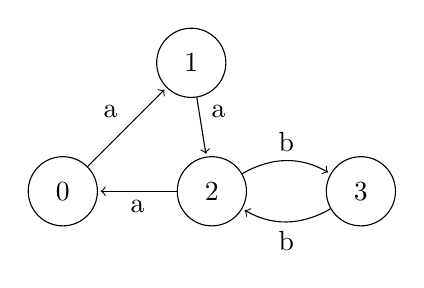
\begin{tikzpicture}[shorten >=1pt,auto]
       \node[state] (q_0)                      {$0$};
       \node[state] (q_1) [above right=of q_0] {$1$};
       \node[state] (q_2) [right=of q_0]       {$2$};
       \node[state] (q_3) [right=of q_2]       {$3$};
        \path[->]
        (q_0) edge  node {a} (q_1)
        (q_1) edge  node {a} (q_2)
        (q_2) edge  node {a} (q_0)
        (q_2) edge[bend left, above]  node {b} (q_3)
        (q_3) edge[bend left, below]  node {b} (q_2);
    \end{tikzpicture}
    \caption{The example of input graph $\mathcal{G}$}
    \label{fig:example_input_graph}
\end{figure}

We use adjacency matrix decomposed to a set of a boolean matrix as a representation of the graph.
\begin{definition}
An adjacency matrix $M$ of the graph $\mathcal{G}=$ is a square $|V|\times|V|$ matrix, such that $M[i,j] = \{l \mid e = (i,l,j) \in E\}$.
\end{definition}

Adjacency matrix $M$ of the graph $\mathcal{G}$ is

$$
    M =
    \begin{pmatrix}
    . & \{a\} & . & .     \\
    . & . & \{a\} & .     \\
    \{a\} & . & . & \{b\} \\
    . & . & \{b\} & .
    \end{pmatrix}.
$$

\begin{definition}

Boolean decomposition of adjacency matrix $M$ of graph $\mathcal{G}=$ is set of Boolean matrix $$\mathcal{M} = \{M^l \mid l \in L, M^l[i,j]=1 \iff l \in M[i,j]\}.$$

\end{definition}

Matrix $M$ can be represented as a set of two Boolean matrices $M^a$ and $M^b$ where
\begin{align}
M^{a} =
\begin{pmatrix}
    . & 1 & . & .   \\
    . & . & 1 & .   \\
    1 & . & . & .   \\
    . & . & . & .  
\end{pmatrix}, 
M^{b} =
\begin{pmatrix}      
    . & . & . & .   \\
    . & . & . & .   \\
    . & . & . & 1   \\
    . & . & 1 & . 
\end{pmatrix} \label{eq:boolean_decomposition_of_graph}
\end{align}
\subsection{Languages}

\begin{definition}\emph{Context-free grammar} is a 4-tuple $G=(N, \Sigma, R, S)$, where 
\begin{itemize}
    \item $N$ is a set of nonterminals
    \item $\Sigma$ is a set of terminals
    \item $R$ is a finite set of productions of the followings form: $A \to \alpha, ~A \in N,~ \alpha \in (N \cup \Sigma)^*$
    \item $S$ - a starting nonterminal
\end{itemize}
\end{definition}

\begin{definition} \emph{Context-free language} is a language generated by a context-free grammar:
\begin{align*}
     L(G) = \{w \in \Sigma^* \mid S \Rightarrow^* w \} 
\end{align*}
Where $S \Rightarrow^* w$  denotes that a string $w$ can be generated from a starting non-terminal $S$ using some sequence of production rules from $P$.
\end{definition}

\begin{definition} Context-free grammar $G = (N, \Sigma, R, S)$ is said to be in \emph{Chomsky normal form} if all productions in $R$ are of the form:
    \begin{itemize}
        \item $A \rightarrow BC,~A,~B,~C \in N$
        \item  $A \rightarrow a,~A \in N,~a \in \Sigma$
        \item $S \rightarrow \varepsilon,~\varepsilon$ is an empty string
    \end{itemize}
\end{definition}
Note that every context-free grammar can be transformed into an equivalent one in Chomsky Normal Form. 
\begin{definition} Context-free grammar $G = (N, \Sigma, P, S)$ is said to be in \emph{Weak Chomsky normal form} if all productions in $P$ are of the form:
    \begin{itemize}
        \item $A \rightarrow BC,~A,~B,~C \in N$
        \item  $A \rightarrow a,~A \in N,~a \in \Sigma$
        \item $A \rightarrow \varepsilon,~A \in N$
    \end{itemize}
\end{definition}
In other words, weak Chomsky normal form differs from Chomsky normal Form in the followings:
\begin{itemize}
    \item $\varepsilon$ can be derived from any non-terminal
    \item $S$ can be at a right part of productions
\end{itemize}
    
    
For example, let's consider the following context-free grammar, which generates the language $L(G) = \{A^nB^n, n \in \mathbb{N}\}$:
$G=(N, \Sigma, P, S), ~N=\{S\},~\Sigma=\{A,B\}$ and productions: 
\begin{align*}
S \rightarrow AB \\
S \rightarrow ASB\\
S \rightarrow \varepsilon
\end{align*}
After transformation to Chomsky Normal Form the resulting grammar:
\begin{align*}
S \rightarrow AB \\
S \rightarrow AC \\
C \rightarrow SB \\
S \rightarrow \varepsilon
\end{align*}

This productions itself are the grammar that has the same result as original grammar.

We use a context-free grammar in the weak Chomsky Normal Form without a starting non-terminal, which will be specified in the path queries for the graph. It should be noted that we omit the rules of the form $A \rightarrow \varepsilon$ for the reason that they correspond to trivial paths, which are more convenient to consider separately.

\begin{definition}\emph{Context-free relation} is a relation $R_A \subseteq V \times V$ for graph $G = (V, E)$, context-free grammar $G = (N,~\Sigma,~P)$ and fixed non-terminal $A$:
\begin{align*}
     R_A = \{(n, m) \mid \exists n \pi m~(l(\pi) \in L(G_A))\}
\end{align*}
\end{definition}

 Now, the definition for \emph{multiple-source (single-source) context-free path querying problem} can be formulated in the introduced notation as follows. For the given graph $G = (V, E)$, context-free grammar $G=(N, \Sigma, P)$ and set of source vertices $Src$ we need to find all context-free relations $R_A$ for any $A \in Src$. 
 
\subsection{Matrix-Based Algorithm}
Let $D = (V, E)$ be the input graph and $G = (N, \Sigma, P)$ be the input grammar. For the context-free path query evaluation, we need to provide context-free relations \mbox{$R_A \subseteq V \times V$} for every \mbox{$A \in N$}.
The matrix-based algorithm for CFPQ can be expressed in terms of operations over Boolean matrices (see listing~\ref{alg:algo0}) which is an advantage for implementation.
{\footnotesize
\begin{algorithm}
\begin{algorithmic}[1]
\caption{Context-free path querying algorithm}
\label{alg:algo0}
\Function{evalCFPQ}{$D=(V,E), G=(N,\Sigma,P)$}
    \State{$n \gets$ |V|}
    \State{$T \gets \{T^{A_i} \mid A_i \in N, T^{A_i}$ is a matrix $n \times n$, $T^{A_i}_{k,l} \gets$ \texttt{false}\} }
    \ForAll{$(i,x,j) \in E$, $A_k \mid A_k \to x \in P$}
        %\Comment{Matrices initialization}
        %\For{$A_k \mid A_k \to x \in P$}
          {$T^{A_k}_{i,j} \gets \texttt{true}$}
        %\EndFor
    \EndFor
    \ForAll{$A_k \mid A_k \to \varepsilon \in P$}
        \ForAll{$i \in \{0,\ldots ,n-1\}$}
            {$T^{A_k}_{i,i} \gets \texttt{true}$}
        \EndFor
    \EndFor

    \While{any matrix in $T$ is changing}
        %\Comment{Transitive c	losure calculation}
        \For{$A_i \to A_j A_k \in P$}
          { $T^{A_i} \gets T^{A_i} + (T^{A_j} \times T^{A_k})$ } 
        \EndFor
    \EndWhile
\State \Return $T$
\EndFunction
\end{algorithmic}
\end{algorithm}
}

This CFPQ algorithm allows efficiently apply GPGPU techniques, but it solves all-pairs problem and takes unreasonable amount of memory in scenarios in which we want to find paths from a relatively small set of vertices, since it calculates a lot of redundant information.  
\section{Matrix-based CFPQ algorithm for all-path query semantics}
\label{sec:all-path-algo}
In this section, we propose the matrix-based algorithm for CFPQ w.r.t. the all-path query semantics (see Listing~\ref{lst:algo1}). This algorithm is a modification of Azimov's matrix-based algorithm for CFPQ and it constructs the set of matrices $T$ with AllPathIndexes as elements.

Let $G = (N, \Sigma, P, S)$ be the input context-free grammar, $D = (V, E, \Sigma)$ be the input graph.
The result of the algorithm is a set of matrices $T$ which stores information about all paths in the graph $D$ that form a word derivable from some nonterminal of the context-free grammar $G$. Note that in line 4 we add the special value $n$ to the $T^{A_i}_{k,l}.middles$ to specify that this path is a single-edge path or an empty path $\pi_{\varepsilon}$.

\begin{algorithm}
\small
\begin{algorithmic}[1]
\floatname{algorithm}{Listing}
\caption{CFPQ algorithm for all-path query semantics}
\label{lst:algo1}
\Function{AllPathCFPQ}{\par
\hskip\algorithmicindent $D = (V, E, \Sigma)$, \par
\hskip\algorithmicindent $G=(N,\Sigma,P,S)$} \Comment{Grammar in WCNF}\par
\State{$n \gets$ |V|}
\State{$T \gets \{T^{A} \mid A \in N, T^{A}$ is a matrix $n \times n$, $T^{A}_{i,j} \gets \bot$ \} }
\ForAll{$(i,x,j) \in E$, $A \mid A \to x \in P$}
%\Comment{Matrices initialization}
%\For{$A_k \mid A_k \to x \in P$}
{$T^{A}_{i,j} \gets (i,j,\{n\})$}
%\EndFor
\EndFor
\ForAll{$A \mid A \to \varepsilon \in P$}
{$T^{A}_{i,i} \gets (i,i,\{n\})$}
\EndFor

\While{any matrix in $T$ is changing}
%\Comment{Transitive closure calculation}
\ForAll{$A \to B C \in P$ where $T^{B}$ or $T^{C}$ are changed}
\State{ $T^{A} \gets T^{A} + (T^{B} \odot T^{C})$ } 
\EndFor
\EndWhile
\State \Return $T$
\EndFunction

\end{algorithmic}
\end{algorithm}

After constructing a set of matrices $T$ or so-called \textit{index}, we can construct a set of all paths $\pi$ between specified vertex pair $(i, j)$ and a non-terminal $A$ such that $A \xLongrightarrow[G]{*} l(\pi)$. The index $T$ already stores data about all paths derivable from each nonterminal. However, the
set of such paths can be infinite. From a practical perspective, it is necessary
to use lazy evaluation or limit the resulting set of paths in some other way.
For example, one can try to query some fixed number of paths or query paths
of fixed maximum length.

We propose the algorithm (see Listing~\ref{lst:algo2}) for extracting these paths. Our algorithm returns a set with the empty path $\pi_{\varepsilon}$ only if $i = j$ and $A \to \varepsilon \in P$. If the AllPathIndex for given $i,j,A$ is equal to $\bot$ then our algorithm returns $\emptyset$ since such paths do not exist. Note that in line 19 we use
the operation $\cdot$ which naturally generalizes the path concatenation operation
by constructing all possible concatenations of path pairs from the given two
sets. It is assumed that the sets are computed lazily, so as to ensure the termination in case of an infinite number of paths.

\begin{algorithm}
	\small
	\begin{algorithmic}[1]
		\floatname{algorithm}{Listing}
		\caption{All paths extraction algorithm}
		\label{lst:algo2}		
		\Function{extractAllPaths}{$i, j, A, T=\{T^{A_i}\}, G=(N,\Sigma,P,S)$}
		\State{$index \gets T^{A}_{i,j}$ }
		
		\If{$index = \bot$}
		\State \Return $\emptyset$
		\Comment{Such paths do not exist}
		\EndIf
		
		\State{$n \gets $ size of the square matrix $T^{A}$}
		\State{$resultPaths \gets \emptyset$}
		
		\ForAll{$middle \in index.middles$}		
		\If{$middle = n$}  \Comment{Add single-edge or empty paths}
		\ForAll{$x \mid A \to x \in P$}
		\If{$(i,x,j) \in E$}
		\State{$resultPaths \gets resultPaths \cup \{((i,x,j))\}$}
		\EndIf
		\EndFor
		\If{$(i = j) \wedge (A \to \varepsilon \in P)$}
		\State{$resultPaths \gets resultPaths \cup \{\pi_{\varepsilon}\}$}
		\EndIf
		\Else \Comment{Add to result the concatenated paths from $i$ to $middle$ and from $middle$ to $j$}
		\ForAll{$A \to B C \in P$}
		\State{$index_B \gets T^{B}_{i,middle}$ }
		\State{$index_C \gets T^{C}_{middle,j}$ }
		\If{$(index_B \neq \bot) \wedge (index_C \neq \bot)$}
		\State{$lPaths \gets$ \Call{extractAllPaths}{$i, middle, B, T, G$}}
		\State{$rPaths \gets$ \Call{extractAllPaths}{$middle, j, C, T, G$}}
		\State{$resultPaths \gets resultPaths \cup lPaths \cdot rPaths$}
		\EndIf
		\EndFor
		\EndIf
		\EndFor
		\State \Return $resultPaths$
		\EndFunction
	\end{algorithmic}
\end{algorithm}

\subsection{Correctness}

The following correctness theorem holds.

\begin{mytheorem}\label{thm:correct}
Let $G = (N, \Sigma, P, S)$ be the input context-free grammar, $D = (V, E, \Sigma)$ be the input graph, and $T$ be a set of matrices returned by the algorithm in Listing~\ref{lst:algo1}. Then for any $i, j$ and for any non-terminal $A \in N$, $index = T^A_{i,j}$ and $index = (i,j,middles) \neq \bot$ iff $(i,j) \in R_{G_A, D}$ and there is a path $\pi$ from vertex $i$ to $j$ such that $l(\pi) \in G_A = (N,\Sigma,P,A)$.
\end{mytheorem}
\begin{proof}[Proof sketch]
	At each iteration of the main cycle in the lines 6-8 of the algorithm, the new paths corresponding to nonterminals $A \in N$ are considered using the rules $A \to B C \in P$. These new paths are obtained by the concatenation of two smaller paths corresponding to the nonterminals $B$ and $C$. At the initialization step of the algorithm in lines 3-5, we consider all single-edge or empty paths corresponding to the derivation tree of height 1. Thus, it can be shown that at iteration $l$ of the main cycle we consider all paths $\pi$ such that there is a derivation tree of the height $h \leq l + 1$ for the string $l(\pi)$ and a context-free grammar $G_A$. Therefore, the theorem can be proved using the induction on the height of such derivation trees.
	
\end{proof}

Now, using the theorem~\ref{thm:correct} and induction on the length of the path, it can be easily shown that the following theorem holds.

\begin{mytheorem}\label{thm:correct_extraction}
Let $G = (N, \Sigma, P, S)$ be the input context-free grammar, $D = (V, E, \Sigma)$ be the input graph, and $T$ be a set of matrices returned by the algorithm in Listing~\ref{lst:algo1}. Then for any $i, j$ and for any non-terminal $A \in N$ such that $index = T^A_{i,j}$ and $index = (i,j,middles) \neq \bot$, the algorithm in Listing~\ref{lst:algo2} for these parameters will return a set of all paths $\pi$ from vertex $i$ to $j$ such that $l(\pi) \in G_A = (N,\Sigma,P,A)$.
\end{mytheorem}

We can, therefore, determine whether $(i,j) \in R_{G, D}$ by asking whether $T^S_{i,j} = \bot$. Also, we can extract all paths which forms a word from the context-free language $L(G)$ by using our algorithm in Listing~\ref{lst:algo2}. Thus, we show how the context-free path query evaluation w.r.t. the all-path query semantics can be solved in terms of matrix operations.

%\subsection{Complexity}

%Denote the number of elementary operations executed by the algorithm of multiplying two $n \times n$ matrices with PathIndexes as $MM(n)$. Also, denote the number of elementary operations, executed by the matrix element-wise + operation of two $n \times n$ matrices with PathIndexes as $MA(n)$. Since the line \textbf{7} of the algorithm in listing~\ref{lst:algo2} is executed no more than $|V|^2|N|$ times (for the same reasons as in the original paper~\cite{Azimov:2018:CPQ:3210259.3210264} of the matrix-based CFPQ algorithm), the following theorem holds.

%\begin{myproposition}\label{thm:time}
%	Let $D = (V,E)$ be a graph and let $G =(N,\Sigma,P)$ be a grammar. The algorithm in listing~\ref{lst:algo2} calculates the set of matrices $T$ in $O(|V|^2|N|^3(MM(|V|) + MA(|V|)))$.
%\end{myproposition}

%Also, denote the time complexity of the access to the PathIndex in the $n \times n$ matrix as $Access(n)$. Then the following theorem on the time complexity of the path extraction algorithm holds.

%\begin{myproposition}\label{thm:time_extraction}
%	Let $D = (V,E)$ be a graph, let $G =(N,\Sigma,P)$ be a grammar and $T$ be a set of matrices returned by the algorithm in listing~\ref{lst:algo2}. Then for any $i, j$ and for any non-terminal $A \in N$ such that $index = T^A_{i,j}$ and $index = (i,j,k,h,l) \neq \bot$, the algorithm in listing~\ref{lst:algo3} for these parameters calculates a path $i \pi j$ in $O(l \times N \times Access(|V|))$.
%\end{myproposition}

\subsection{An Example}
In this section, we provide a step-by-step demonstration of the proposed algorithms. %For this, we consider the example with the worst-case time complexity.

We run the query on a graph $D_1$, presented in Figure~\ref{fig:example_input_graph}. We provide a step-by-step demonstration of the work of algorithm in Listing~\ref{lst:algo1} with the given graph $D$ and grammar $G_1^{\text{wcnf}}$ from section~\ref{sec:preliminaries}. After the matrix initialization in lines \textbf{3-5} of this algorithm, we have a set of matrices $T^{(1)}$, presented in Figure~\ref{ExampleQueryInitMatrix}.

{\footnotesize
	\begin{figure}[h]
		\[
		T^{(1),A} = \begin{pmatrix}
			\bot & (0,1,\{4\})       & \bot & \bot       \\
			\bot & \bot & (1,2,\{4\})       & \bot \\
			(2,0,\{4\})       & \bot & \bot & \bot \\
			\bot       & \bot & \bot & \bot \\
		\end{pmatrix}
		\]
		\[
		T^{(1),B} = \begin{pmatrix}
			\bot & \bot       & \bot & (0,3,\{4\})       \\
			\bot & \bot & \bot       & \bot \\
			\bot       & \bot & \bot & \bot \\
			(3,0,\{4\})      & \bot & \bot & \bot \\
		\end{pmatrix}
		\]
		\caption{The initial matrices for the example query. The PathIndexes $T^{(1),S_1}_{i,j}$ and $T^{(1),S}_{i,j}$ are equal to $\bot$ for every $i,j$}
		\label{ExampleQueryInitMatrix}
	\end{figure}
}

After the initialization, the only matrices which will be updated are $T^{S_1}$ and $T^{S}$. These matrices obtained after the first loop iteration is shown in Figure~\ref{ExampleQueryFirstIteration}.

{\footnotesize
	\begin{figure}[h]
		\[
		T^{(2),S} = \begin{pmatrix}
			\bot & \bot       & \bot & \bot       \\
			\bot & \bot & \bot       & \bot \\
			\bot       & \bot & \bot & (2,3,\{0\}) \\
			\bot       & \bot & \bot & \bot \\
		\end{pmatrix}
		\]
		\caption{The first iteration of computing the transitive closure for the example query. The PathIndexes $T^{(1),S_1}_{i,j}$ are equal to $\bot$ for every $i,j$}
		\label{ExampleQueryFirstIteration}
	\end{figure}
}

When the algorithm at some iteration finds new paths for some non-terminal in the graph $D_1$, then it adds corresponding AllPathIndexes to the matrix for this non-terminal. For example, after the first loop iteration, AllPathIndex $(2,3,\{0\})$ is added to the matrix $T^{S}$. This AllPathIndex is added to the element with a row index $i = 2$ and a column index $j = 3$. This means, that there is a path $\pi$ from the vertex 2 to the vertex 3, such that $S \xLongrightarrow[G_1^{\text{wcnf}}]{*} l(\pi)$ and this path obtained by concatenation of two smaller paths via vertex 0.

The calculation of the index $T$ is completed after $k$ iterations, when a fixpoint is reached: $T^{(k)} = T^{(k-1)}$. For the example query, $k = 14$ since $T_{14} = T_{13}$. The resulted matrix for non-terminal $S$ is presented in Figure~\ref{ExampleQueryFinalMatrices}.

{\footnotesize
	\begin{figure}[h]
		\[
		T^{(14),S} = \begin{pmatrix}
			(0,0,\{1\}) & \bot       & \bot & (0,3,\{1\})       \\
			(1,0,\{2\}) & \bot & \bot       & (1,3,\{2\}) \\
			(2,0,\{0\})       & \bot & \bot & (2,3,\{0\}) \\
			\bot       & \bot & \bot & \bot \\
		\end{pmatrix}
		\]
		\caption{The final matrix for non-terminal $S$ after computing the index}
		\label{ExampleQueryFinalMatrices}
	\end{figure}
}

Now, after constructing the index, we can construct the context-free relation $$R_{G_1^{\text{wcnf}}, D_1}=\{(0,0),(0,3),(1,0),(1,3),(2,0),(2,3)\}.$$

In the relation $R_{G_1^{\text{wcnf}}, D_1}$, we have all vertex pairs corresponding to paths, whose labeling is in the language $L(G_1^{\text{wcnf}}) = \{a^n b^n \mid n \geq 1\}$. Using the algorithm in Listing~\ref{lst:algo2} we can restore paths for each vertex pair from the context-free relation. For example, given $i=j=0$, non-terminal $S$, set of resulted matrices $T$, and context-free grammar $G_1^{\text{wcnf}}$, the algorithm in Listing~\ref{lst:algo2} returns an infinite set of all paths from vertex 0 to vertex 0 whose labeling form words from the following set $\{a^6 b^6, a^{12} b^{12}, a^{18} b^{18}, \ldots \}$. Following the path corresponding to the word $a^{6m} b^{6m}$, we will go through the cycle with $a$ labels $2m$ times and through the cycle with $b$ labels $3m$ times for all $m \geq 1$.
\section{Evaluation}

This section describes the methodology and answers the following research questions.

\begin{enumerate}
    \item Does fusion via distillation give any benefits at the software and hardware levels?
    \item What are the properties of the generated hardware?
    \item Does the generated hardware outperform software implementations?
\end{enumerate}

\subsection{Methodology}

Our focus is on creating a basis for future research and experiments, thus we make our experiments as much reproducible as possible\footnote{\url{https://github.com/sedwards-lab/fhw/tree/sparse-linear-algebra-distillation/examples/QTreeBenchmarks/diploma/verilog-bool-no-nnz-inlined} (online; accessed:
2022-06-07) Here one could find all the results. For each benchmark all statistics are specified: matrix names, their sizes, collected metrics for both hardware and software benchmarks.}. We benchmarked the following list of chained functions. The choice is prompted by the current state of the distiller: at the moment, it does not successfully distill matrix multiplication. However, the functions are still practical enough, for example, chained addition could be seen in Luby's maximal independent set algorithm and clearly describe the applicability of the proposed approach.

\begin{itemize}
    \item \mintinline{Haskell}{mAdd (==False) (||) (mAdd (==False) (||) m1 m2) m3}
    \item \mintinline{Haskell}{mask (mAdd (== False) (||) m2 m3) (m1)}
    \item \mintinline{Haskell}{map (==Zero) (to_nat) (mAdd (==False) (||) m1 m2}
    \item \mintinline{Haskell}{map (==Zero) (to_nat) (kron (==False) (&&) m1 m2}
\end{itemize}

Above, \mintinline{Haskell}{Zero} and \texttt{to\_nat} are corresponding definitions for Peano arithmetics, since the \texttt{.pot} language does not have any primitives. For the same reason, we operated with boolean matrices. Such functions could be abstracted with free variables and then instantiated in the emitted Haskell code. However, to get maximum from distillation, we provided all the information about the functions. 

For these functions, we compared the execution time of distilled and not distilled hardware generated circuits, execution time of original and distilled Haskell code and reference \textit{Suite Sparse}\footnote{\url{https://github.com/DrTimothyAldenDavis/GraphBLAS} (online; accessed:
2022-06-07), Suite Sparse library sources.}\textsuperscript{,}\footnote{The library also uses different variations of coordinate formats (opaque to the user) and not a quadtree representation.} variants of these functions in C\texttt{++}. Note that SuiteSparse does not support recursive data types, thus only the first two function chains were implemented in SuiteSparse (since Peano number is essentially a linked list). We did not replace Peano numbers with integers, so our experiments could be interpreted easier. For hardware experiments we collected execution time and the number of memory writes and reads, to access how well fusion is performed. For software experiments we only measured the execution time. Also note that we measured only the time, required to execute the lines above, not including any IO, required to get and evaluate function arguments. But in hardware benchmarks we measured the time required to pass arguments into the circuit's memory, because such IO is inevitable. It is tricky to make such measures in Haskell due to laziness, thus the programs were compiled with \texttt{--fno-full-laziness} to turn off memoization. Also all the arguments were forced to normal form via \texttt{force} and \texttt{evaluate}. Haskell programs were compiled\footnote{GHC 8.10.4.} with \texttt{-O2 --fno-full-laziness} and Suite Sparse was compiled with default flags and linked as a shared library to C\texttt{++} code.

We took matrices from SuiteSparse matrix collection with sizes ranging from \texttt{64x64} to \texttt{512x512}. We limited ourselves with such sizes due to the fact that this is the maximum sizes that fit into \texttt{bram} with $2^{16}$ address space. Such number of \texttt{bram} blocks is available only on really expensive FPGA boards, thus in practice sizes would be smaller to achieve better utilization. Once again, it models the situation when data fits into the cache, since \texttt{bram} in our circuits will operate as a cache in real application.

\subsection{Experiments}

Table~\ref{tab:bench_results} shows the results of all execution time benchmarks. To evaluate execution time for hardware simulation, implementation stage was performed to assess the maximum frequency of FPGA device used for synthesis and implementation, and the number of execution cycles was multiplied by the number of nanoseconds a clock cycle takes. The frequencies were equal within the same benchamark set, i.e., frequency was not affected by distillation. We used \texttt{xcu250figd2104-2L} device\footnote{\url{https://www.xilinx.com/products/boards-and-kits/alveo/u250.html}  (online; accessed:
2022-06-07)} for synthesis and implementation stages. It is not really a casual and affordable chip, but it contains enough \texttt{bram} for our evaluation to see scalability. In the table a median across several benchmarks is shown. 

As it could be seen, distillation steadily increases performance: up to 2x speedup for hardware simulation and up to 3x for software benchmarks. The results are maintained within the borders of the corresponding confidence interval and the borders are not shown for brevity. Hardware speedup is lower due to the different execution semantics, dataflow is not reduction-based and distillation is a reduction-based transformation. Note that generated hardware appears to be less performant than both Haskell and C\texttt{++}, which a bit contradicts the results from~\cite{oldfhw}. For hardware benchmarks \texttt{time (IO)} shows the execution time including the time needed to transfer the data though the arguments, \texttt{time (no IO)} does not include it in its turn. It could be seen that not all the benchmarks are computationally extensive enough to cover memory transferring costs, but for more complex examples the ratio would be better. Since we basically transfer the matrices node by node from a file in the testbench, we have probably the lowest possible latency, and in practice it would be higher if reading from DDR, however the bandwidth could be increased. Noticeably, running times for \texttt{mMaskAdd} for C\texttt{++} and distilled Haskell are similar, which shows that fusion really provides some extra performance: SuiteSparse at the moment does not implement any fusion.

Table~\ref{tab:mem_results} summarizes the ratios between distilled and not distilled hardware circuits memory reads and writes. Since in general case distillation removes extra pattern matching, essentially it saves memory reads and writes. The eventual number of memory reads and writes is implementation dependent, thus the table shows what share of speedup is prompted by saving memory operations. Distillation successfully reduces the number of memory accesses, about 15\% on average. \texttt{mMapKron} has a bit higher ratio due to the fact that \texttt{Nat} numbers require additional memory accesses, since the type is recursive. It could also be seen that a major part of speedups is attributed to saved memory accesses. 

Finally, table~\ref{tab:resource_util} shows device resources utilization ratios between distilled and not distilled hardware circuits and frequencies. Columns are device primitives: registers, lookup tables, \texttt{bram} blocks or multiplexers. Utilization for both types of circuits is below 1\% of available resources on the device, except for the memory. Memory blocks utilization is about 30\% (since we choose larger \texttt{brams} to store larger matrices). Apart from that, distilled circuits could have both higher and lower utilization. Since the hardware generation is primarily syntax-directed it follows from the distilled program structure. For example, distillation might glue two recursive functions into one (in that case, memory utilization would be lower, because each cluster of mutually recursive functions possesses its own heap) or make more recursive functions than in the original program. The frequencies are the same, however, they possibly could be made better with more intelligent buffer allocation.

\subsection{Discussion}
Answering the research questions above.

\begin{enumerate}
    \item Fusion gives significant benefits, however at the hardware level the benefits are a bit smaller since hardware semantics is not reduction based. The benefits at the hardware level are mostly determined by the reduced number of memory accesses (each access takes 2 clock cycles). Notably, distilled Haskell implementation of \texttt{mMaskAdd} has similar performance with C\texttt{++}. 
    \item Device utilization is low, but such circuits could be copied on the same device to provide better utilization and higher parallelism. Resource utilization might be both better and worse after distillation, depending on the transformed program itself since translation is syntax-directed. Frequency could be increased by more intelligent buffering strategy.
    \item Although we use low-latency design with \texttt{bram}s that take 2 clock cycles per request and transfer matrices from files, which does not have any latency in simulation, we get slower execution time than Haskell and C\texttt{++} counterparts. It could be partly due to excessive buffering performed by FHW at the moment. Also there is no pipelining for recursive calls, i.e. only one set
of function argument tokens are allowed to enter a tail-recursive function call until a result is finally generated. Further CPS transformation hinders parallelization, which could be made more explicit with SSA. Some other optimizations exist that may significantly influence the performance. Also, since device utilization is about 1\%, such circuits could be copied on one device and provide more parallelism. A more detailed discussion could be found at~\cite{Edwards2019FHWP}.
\end{enumerate}

Distillation clearly showed its applicability to optimization of sparse linear algebra routines and notably it still could be combined with other techniques, like rewrite rules to achieve better results. High-level synthesis has a room for improvements by increasing pipelining, parallelism and frequency and the generated hardware could be improved from usability perspective: a support for arbitrary sized matrices is desirable. Thus we will focus on these directions. Probably a better solution would be to embed \texttt{.pot} language into e.g. Haskell to leverage its type system (to be able to use some rewrite rules as well), and add support for primitive types and parallel primitives to be able to conduct a more scalable comparison with SuiteSparse (since SuiteSparse is multithreaded). For such embedding different execution models could be implemented, including hardware synthesis, for which SSA form of GRIN looks promising, as well as extra optimizations shipped with GRIN. For hardware synthesis, an interesting direction is achieving predictable results in hardware from certain modifications in software. This property partly holds for the current approach, since the translation is syntax- directed. More information on this could be found at~\cite{predict}.

\pagebreak

\begin{table}[t]
\scriptsize
\centering
\caption*{mAddAdd}
\begin{tabular}{|c|c|c|c|c|c|c|c|c|c|} 
\hline
\rowcolor{LightBlue}
\multicolumn{3}{|c|}{Matrices dimensions} & Haskell & Haskell (distilled) & \multicolumn{2}{c|}{FHW} & \multicolumn{2}{c|}{FHW (distilled)} & {C\texttt{++}}\\
% \rowcolor{LightBlue}
\hline
m1 & m2 & m3 & time & time & time (no IO) & time (IO) & time (no IO) & time (IO) & time \\ 
\hline
64 & 64 & 64 & 29 us & 20 us & 76 us & 170 us & 64 us & 158 us & 14 us\\ 
128 & 128 & 128 & 94 & 79 & 146 & 476 & 134 & 469 & 30 \\
256 & 256 & 256 & 123 & 103 & 202 &  681 & 168 & 662 & 44\\
512 & 512 & 512 & 219 & 143 & 474 & 1192 & 375 & 1093 & 49\\
\hline
\end{tabular}

\caption*{mMaskAdd}
\begin{tabular}{|c|c|c|c|c|c|c|c|c|c|} 
\hline
\rowcolor{LightBlue}
\multicolumn{3}{|c|}{Matrices dimensions} & Haskell & Haskell (distilled) & \multicolumn{2}{c|}{FHW} & \multicolumn{2}{c|}{FHW (distilled)} & {C\texttt{++}}\\
% \rowcolor{LightBlue}
\hline
m1 & m2 & m3 & time & time & time (no IO) & time (IO) & time (no IO) & time (IO) & time \\ 
\hline
64 & 64 & 64 & 10 us & 7 us & 64 us & 133 us & 46 us & 111 us & 18 us\\ 
128 & 128 & 128 & 38 & 30 & 118 & 322 & 75 & 292 & 33 \\
256 & 256 & 256 & 48 & 42 & 168 &  498 & 104 & 456 & 46\\
512 & 512 & 512 & 126 & 76 & 400 & 762 & 300 & 729 & 65\\
\hline
\end{tabular}

\caption*{mMapAdd}
\begin{tabular}{|c|c|c|c|c|c|c|c|c|c|} 
\hline
\rowcolor{LightBlue}
\multicolumn{3}{|c|}{Matrices dimensions} & Haskell & Haskell (distilled) & \multicolumn{2}{c|}{FHW} & \multicolumn{2}{c|}{FHW (distilled)} & {C\texttt{++}}\\
% \rowcolor{LightBlue}
\hline
m1 & m2 & m3 & time & time & time (no IO) & time (IO) & time (no IO) & time (IO) & time \\ 
\hline
64 & 64 & --- & 45 us & 37 us & 189 us & 253 us & 137 us & 202 us & ---\\ 
128 & 128 & --- & 162 & 105 & 524 & 685 & 397 & 579 & --- \\
256 & 256 & --- & 312 & 216 & 1047 &  1360 & 680 & 986 & ---\\
512 & 512 & --- & 436 & 273 & 1346 & 1776 & 900 & 1330 & ---\\
\hline
\end{tabular}

\caption*{mMapKron}
\begin{tabular}{|c|c|c|c|c|c|c|c|c|c|} 
\hline
\rowcolor{LightBlue}
\multicolumn{3}{|c|}{Matrices dimensions} & Haskell & Haskell (distilled) & \multicolumn{2}{c|}{FHW} & \multicolumn{2}{c|}{FHW (distilled)} & {C\texttt{++}}\\
% \rowcolor{LightBlue}
\hline
m1 & m2 & m3 & time & time & time (no IO) & time (IO) & time (no IO) & time (IO) & time \\ 
\hline
2 & 64 & --- & 64 us & 36 us & 212 us & 242 us & 94 us & 125 us & ---\\ 
2 & 128 & --- & 137 & 68 & 434 & 502 & 199 & 266 & --- \\
2 & 256 & --- & 364 & 126 & 1004 &  1188 & 449 & 636 & ---\\
4 & 128 & --- & 302 & 94 & 694 & 763 & 330 & 401 & ---\\
\hline
\end{tabular}



\caption{Execution time}
\label{tab:bench_results}

\end{table}
\begin{table}[h]
\scriptsize
\begin{minipage}{0.45\linewidth}
\centering
\caption*{mAddAdd}
\begin{tabular}{|c|c|c|c|c|c|c|} 
\hline
\rowcolor{LightBlue}
\multicolumn{3}{|c|}{Matrices dimensions} & \multicolumn{2}{c|}{Ratio ($\frac{FHW}{FHW_{distilled}}$)}\\
% \rowcolor{LightBlue}
\hline
m1 & m2 & m3 & writes & reads\\ 
\hline
64 & 64 & 64 & 1.10 & 1.15\\ 
128 & 128 & 128 & 1.02 & 1.05\\
256 & 256 & 256 & 1.03 & 1.06\\
512 & 512 & 512 & 1.10 & 1.16\\
\hline
\end{tabular}
\end{minipage}
\begin{minipage}{0.45\linewidth}
\centering
\caption*{mMaskAdd}
\begin{tabular}{|c|c|c|c|c|c|c|} 
\hline
\rowcolor{LightBlue}
\multicolumn{3}{|c|}{Matrices dimensions} & \multicolumn{2}{c|}{Ratio ($\frac{FHW}{FHW_{distilled}}$)}\\
% \rowcolor{LightBlue}
\hline
m1 & m2 & m3 & writes & reads\\ 
\hline
64 & 64 & 64 & 1.13 & 1.26\\ 
128 & 128 & 128 & 1.06 & 1.11\\
256 & 256 & 256 & 1.08 & 1.09\\
512 & 512 & 512 & 1.10 & 1.16\\
\hline
\end{tabular}
\end{minipage}
\begin{minipage}{0.45\linewidth}
\centering
\caption*{mMapAdd}
\begin{tabular}{|c|c|c|c|c|c|c|} 
\hline
\rowcolor{LightBlue}
\multicolumn{3}{|c|}{Matrices dimensions} & \multicolumn{2}{c|}{Ratio ($\frac{FHW}{FHW_{distilled}}$)}\\
% \rowcolor{LightBlue}
\hline
m1 & m2 & m3 & writes & reads\\ 
\hline
64 & 64 & --- & 1.10 & 1.21\\ 
128 & 128 & --- & 1.07 & 1.14\\
256 & 256 & --- & 1.07 & 1.19\\
512 & 512 & --- & 1.10 & 1.21\\
\hline
\end{tabular}
\end{minipage}
\hfill
\begin{minipage}{0.45\linewidth}
\centering
\caption*{mMapKron}
\begin{tabular}{|c|c|c|c|c|c|c|} 
\hline
\rowcolor{LightBlue}
\multicolumn{3}{|c|}{Matrices dimensions} & \multicolumn{2}{c|}{Ratio ($\frac{FHW}{FHW_{distilled}}$)}\\
% \rowcolor{LightBlue}
\hline
m1 & m2 & m3 & writes & reads\\ 
\hline
2 & 64 & --- & 1.71 & 1.88\\ 
2 & 128 & --- & 1.72 & 1.87\\
2 & 256 & --- & 1.65 & 1.83\\
4 & 128 & --- & 1.81 & 1.91\\
\hline
\end{tabular}
\end{minipage}

\caption{Memory accesses}
\label{tab:mem_results}
\end{table}

\begin{table}[h]
\scriptsize
\centering
\begin{tabular}{|l|c|c|c|c|c|c|c|c|c|} 
\hline
\rowcolor{LightBlue}

{Benchmark} & \multicolumn{8}{c|}{Ratio (${\frac{FHW}{FHW_{distilled}}}$)} & {Frequency}\\
\hline
{} & FDRE & LUT3 & LUT6 & LUT5 & LUT4 & LUT2 & RAMB36E2 & MUXF7 & {} \\
% \rowcolor{LightBlue}
\hline
mAddAdd & 0.3 & 0.3 & 0.3 & 0.5 & 0.3 & 0.3 & 0.5 & 0.5 & 200 MHz\\ 
mMaskAdd & 0.5 & 0.5 & 0.7 & 0.4 & 0.7 & 0.5 & 0.7 & 0.6 & 200 MHz\\
mMapAdd & 1 & 0.9 & 0.9 & 1.2 & 1 & 1.1 & 1.1 & 1.2 & 200 MHz\\
mMapKron & 1.5 & 1.5 & 1.3 & 2 & 2 & 1.8 & 1.4 & 1.7 & 200 MHz\\
\hline
\end{tabular}
\caption{Resource utilization}
\label{tab:resource_util}
\end{table}
\pagebreak

\section{Conclusion and Future Work}

We present !!!

Our evaluation shows that !!!

First direction for future research is a more detailed CFPQ algorithms investigation.
We should do More evaluation on sparse matrices on GPGPUs.

Also it is nesessary to implement and evaluate solutions for graphs which is not fit in RAM.
There is a set of technics for huge matrices multiplication.
Is it possible to dopt it for CFPQ

Another direcion is a dataset improvement.
More data.
More grammars/queries.


\begin{acks}
	The reported study was funded by RFBR, project number 19-37-90101, and grant from JetBrains Research.
\end{acks}

%\section*{Acknowledgements}
%The research was supported by the Russian Science Foundation, grant \textnumero 18-11-00100.

%We thank Roi Lipman for his help with investigation of the RedisGraph internals and pointing out the impractical memory consumption of the original Azimov's algorithm which gave us the motivation to develop the presented solution.

%We thank Ekaterina Verbitskaia for the fruitful discussion and feedback which helped us to improve the paper.

%Anonimus reviewers !!!

\balance

%%
%% The next two lines define the bibliography style to be used, and
%% the bibliography file.
\bibliographystyle{ACM-Reference-Format}
\bibliography{all-path-matrix-cfpq}

%%
%% If your work has an appendix, this is the place to put it.
%% Please note that all the content must fit within the page limits, including any appendices.
%\appendix
%
%\section{Research Methods}
% ...

\end{document}
\endinput




